\documentclass[12pt, letterpaper]{article}
\usepackage{amsmath}
\usepackage{amssymb}
\usepackage{graphicx} 
\title{STA 630 - Homework 1}
\author{Anthony Bernardi}
\date{January 31, 2025}
\begin{document}
\maketitle

\section{Problem 1 - Hoff 2.3}

\subsection{Part A}

Let X, Y, Z be random variables with joint density $p(x, y, z)$ which is proportional to $f(x, z) g(y, z) h(z)$. 

Show the following. 

\begin{equation} 
p(x | y, z) \propto f(x, z) 
\end{equation} 

We will do this with the definition of conditional probability. 

\begin{equation}
p(x | y, z) = \frac{p(x, y, z)}{p(y, z)} 
\end{equation} 

We can now re-write this in the following way. 

\begin{equation} 
\frac{p(x, y, z)}{p(y, z)} \propto f(x, z)
\end{equation}

We can continue re-writing to get something more workable. 

\begin{equation}
\frac{f(x, z) g(y, z) h(z)}{p(y , z)} \propto f(x, z) 
\end{equation} 

We can now continue to re-write until the cancellation becomes apparent. 

\begin{equation} 
\frac{f(x, z) g(y, z) h(z)}{g(y, z) h(z)} \propto f(x, z) 
\end{equation} 

We can now see that the g(y, z) and h(z) terms cancel out, and the final result is apparent. 

\begin{equation} 
p(x | y, z)  = f(x, z) \propto f(x, z) 
\end{equation} 

\subsection{Part B} 

Show the following. 

\begin{equation}
p(y | x, z) \propto g(y, z) 
\end{equation} 

We can do this in a similar way to part A, relying on the definition of conditional probability. 

\begin{equation} 
p(y | x, z) = \frac{p(x, y, z)}{p(x, z)} 
\end{equation} 

We'll now re-write. 

\begin{equation} 
\frac{p(x, y, z)}{p(x, z)} \propto g(y, z) 
\end{equation} 

Again, we can re-write to make the cancellation more apparent. 

\begin{equation} 
\frac{f(x, z) g(y, z) h(z)}{p(x, z)} \propto g(y, z)
\end{equation} 

Our final step and the cancellation becomes clear. 

\begin{equation} 
\frac{f(x, z) g(y, z) h(z)}{f(x, z) h(z)} \propto g(y, z) 
\end{equation} 

This cancels to reveal the following. 

\begin{equation} 
p(y | x, z) = g(y, z) \propto g(y, z) 
\end{equation} 

\subsection{Part C} 

Show that X and Y are conditionally independent given Z. 

We will use the proportionality provided earlier to establish this. We will start with the definition of conditional independence. 

\begin{equation} 
p(x, y | z) = p(x | z) p(y | z) 
\end{equation} 

We can now re-write this from the definition of conditional probability. 

\begin{equation} 
\frac{p(x, y, z)}{p(z)} = \frac{p(x, z)}{p(z)} \frac{p(y, z)}{p(z)} 
\end{equation} 

We can now simplify this before considering the proportionality. 

\begin{equation} 
\frac{p(x, y, z)}{p(z)} = \frac{p(x, z) \cdot p(y, z)}{p(z)^2} 
\end{equation} 

Now we can use the proportionality to simplify this and get our result. 

\begin{equation}
\frac{f(x, z) g(y, z) h(z)}{h(z)} = \frac{f(x, z) h(z)}{h(z)} \frac{g(y, z) h(z)}{h(z)} 
\end{equation} 

Now we can see how this simplifies to the following. 

\begin{equation} 
f(x, z) g(y, z) = f(x, z) g(y, z) 
\end{equation} 

This shows that X and Y are conditionally independent given Z. 

\section{Problem 2}

Suppose that 6 observations are taken at random from a uniform distribution on the interval $(\theta - .5 , \theta + .5)$, with $\theta$ unknown, and we observe the following values. $(11.0, 11.5, 11.7, 11.1, 11.4, 10.9)$. 

Suppose the prior distribution of $\theta$ is uniform on the interval $(10, 20)$.

Derive the posterior of $\theta$. 

We will do this by first finding the likelihood function, and then multiplying this by the prior to derive our posterior function. 

The likelihood function is given by the following. 

\begin{equation}
L(\theta) = \prod_{i=1}^{6} \frac{1}{\theta + .5 - \theta + .5} = \frac{1}{(\theta + .5)^6 - (\theta - .5)^6} 
\end{equation} 

The prior is given by the following. 

\begin{equation} 
p(\theta) = \frac{1}{20 - 10} = \frac{1}{10} 
\end{equation} 

The posterior is given by the following. 

\begin{equation} 
p(\theta | x) \propto L(\theta) p(\theta) 
\end{equation} 

We can now plug in our likelihood and prior to get the following. 

\begin{equation}
p(\theta | x) \propto \frac{1}{(\theta + .5)^6 - (\theta - .5)^6} \frac{1}{10} 
\end{equation} 

We can now simplify this to get the following. 

\begin{equation} 
p(\theta | x) \propto \frac{1}{10((\theta + .5)^6 - (\theta - .5)^6)} 
\end{equation} 

If we want to get more specific, we can say the following regarding the distribution of the posterior. 

\begin{equation} 
p(\theta | x) \sim Uniform(10 * ((\theta + .5) - (\theta - .5)^6))
\end{equation} 

\section{Problem 3}

Suppose we are going to sample 100 individuals from a larger population, and we are asking if each individual person if they support policy Z or not. Let $Y_i = 1$ if they support the policy and $Y_i = 0$ if they do not. 

\subsection{Part a}

Assume $Y_1, Y_2, ..., Y_{100}$ are independent and identically distributed with $Y_i \sim Bernoulli(\theta)$, where $\theta$ is the proportion of the population that supports the policy. 

Write down the joint distribution of $P(Y_1 = y1, Y_2 = y2, ..., Y_{100} = y100 | \theta)$ in a compact form. Also, write down the form of $P(\sum Y_i = y | \theta)$. 

We can write the joint distribution in the following way, given the Bernoulli distribution. 

Given that we are looking for an exact value for each of the 100 individuals, we can write the joint distribution as the following. 

\begin{equation}
P(Y_1 = y1, Y_2 = y2, ..., Y_{100} = y100 | \theta) = \prod_{i=1}^{100} \theta^{y_i} (1 - \theta)^{1 - y_i} 
\end{equation} 

We will now handle the sum, which we can think about as the sum of the Bernoulli random variables, which is a binomial distribution. 

\begin{equation} 
P(\sum Y_i = y | \theta) = \binom{100}{y} \theta^y (1 - \theta)^{100 - y} 
\end{equation} 

\subsection{Part b} 

For a moment, suppose you believed that the parameter $\theta$ had the following characteristic. $\theta \in$ {0, 0.1, ..., 0.9, 1.0}. 

Given that the results of the survey were $\sum_{i=1}^100 Y_i = 57$, compute $P(\sum Y_i = 57 | \theta)$ for each of these 11 values and plot these probabilities as a function of $theta$. 

Given this information, we can use the Binomial distribution for each possible parameter value in the parameter space, and plot the outputs of these probabilities with R. 

The following code was used to generate the values, and the plot is attached. 

\begin{verbatim}
theta_v <- seq(0, 1, by = 0.1) 

# fixed values 
x <- 57 
n < 100 
likelihoods <- vector(length = 11) 

for (param in theta_v){
  i = 0 
  likelihoods[i] <- dbinom(x, n, param) 
  i = i + 1 
}

plot(x = theta_v , 
     y = likelihoods, 
     type = "l", 
     xlab = "Theta", 
     ylab = "P(Y = 57 | Theta)", 
     main = "Probability of Y = 57 for different values of Theta")
\end{verbatim}

\begin{figure}
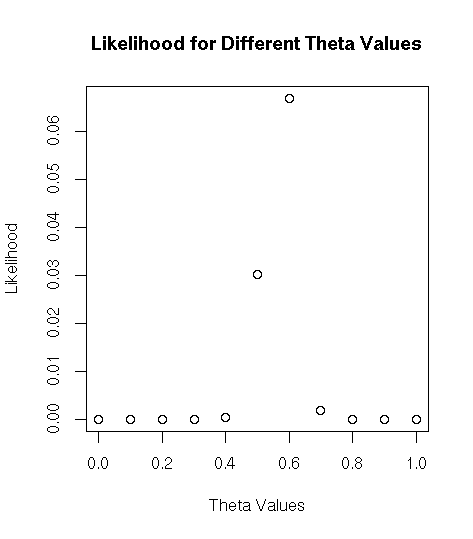
\includegraphics[scale=.5]{/home/adbucks/Documents/sta_630/Likelihood_plot_3.1b.png}
\end{figure}

\subsection{Part c} 

Now suppose you had no prior information to believe one of these $\theta$ values over another, and they were all equally probable. Use Bayes' rule to compute $P(\theta | \sum_{i=1}^100 Y_i = 57)$ for each $\theta$ value. Make a plot of the posterior distribution as a function of $\theta$. 

Using the prior code as a starting point, we can demonstrate how we might simulate the posterior distribution in this case. The following Python code shows how. 

\begin{verbatim}
# using bayes formula assuming equal probabilities for each theta 
prior = [1/11 for i in range(11)]
complement = [1 - i for i in prior] 
likelihood = binom_probs 

# can now do this for each theta and its complement 
posterior = [prior[i] * likelihood[i] /
(prior[i] * likelihood[i] + complement[i] *
(1 - likelihood[i])) for i in range(11)]
print("Posterior Probabilities: ", posterior)

# can now plot these and find the max 
plt.plot(theta_space , posterior) 
plt.xlabel('Theta') 
plt.ylabel('Posterior Probability') 
plt.title('Posterior Probabilities for x = 57, n = 100') 
plt.show() 
\end{verbatim} 

\begin{figure} 
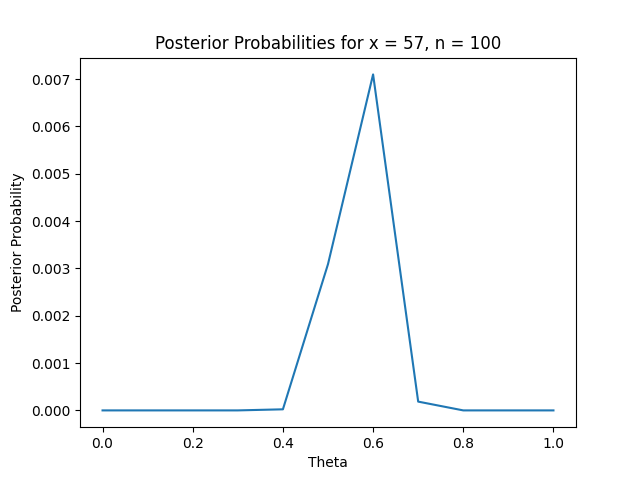
\includegraphics[scale=.5]{/home/adbucks/Documents/sta_630/posterior_plot_31c.png}
\end{figure} 

\subsection{Part d}

Now suppose you allow $\theta$ to be any value in the interval [0,1]. Using the uniform prior density for $\theta$, such that $p(\theta) = 1$, plot the posterior density as a function of $\theta$. 

Given the uniform prior, we can use the following code to simulate the posterior distribution, with a different posterior calculation emphasizing the likelihood, given the "flat" prior of 1. 

\begin{verbatim} 
# trying the posterior again, with theta on an interval from [0,1]
theta_space_c = np.linspace(0,1, 1000) # approximation for continuous 
binom_probs_c = [stats.binom.pmf(x, n, theta) for theta in theta_space_c] 

# now we can plot 
plt.plot(theta_space_c, binom_probs_c) 
plt.xlabel('Theta') 
plt.ylabel('Binomial Probability') 
plt.title('Binomial Probabilities for x = 57, n = 100') 
plt.show() 
\end{verbatim} 

The plot for the posterior distribution in this case is included here. 

\begin{figure} 
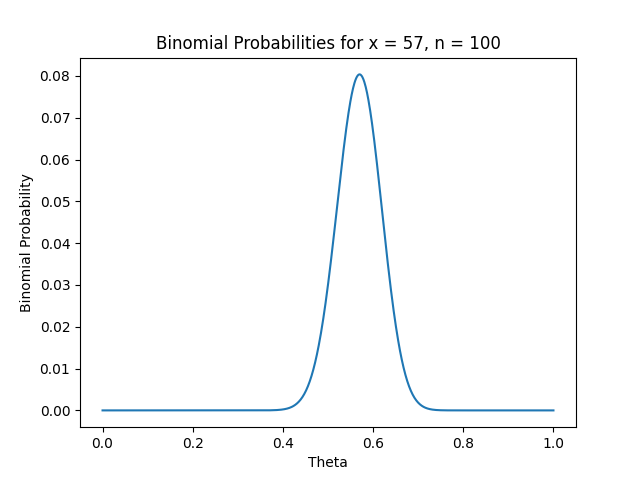
\includegraphics[scale=.5]{/home/adbucks/Documents/sta_630/posterior_plot_31d.png}
\end{figure} 

\subsection{Part e} 

As discussed in this chapter, the posterior distribution of $\theta$ is beta distributed $beta(1 + 57, 1 + 100 - 57)$. Plot the posterior density as a function of $\theta$. Discuss the relationships among all the plots. 

Given the beta distribution, we can use the following code to simulate the posterior distribution. 

\begin{verbatim}
# can recycle our theta space 
alpha = 1 + 57 
beta = 1 + 100 - 57 

# calculating the beta posterior 
beta_posterior = [stats.beta.pdf(theta, alpha, beta) 
for theta in theta_space_c]

# now can plot with theta on the x axis 
plt.plot(theta_space_c, beta_posterior) 
plt.xlabel('Theta') 
plt.ylabel('Beta Posterior') 
plt.title('Beta Posterior for x = 57, n = 100') 
plt.show() 
\end{verbatim} 

Here is the plot as shown by the code. 

\begin{figure} 
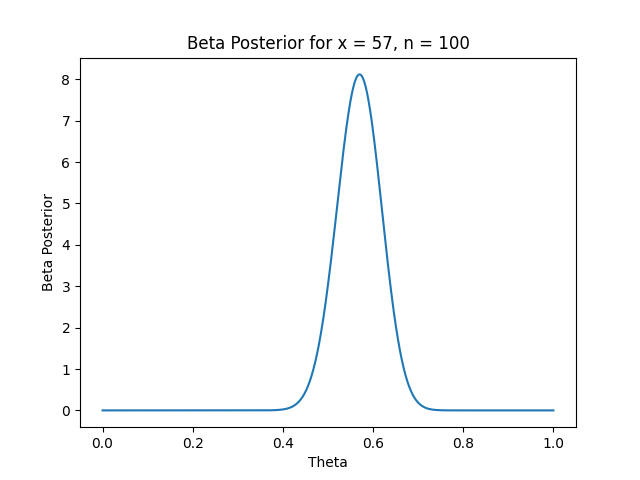
\includegraphics[scale=.5]{/home/adbucks/Documents/sta_630/beta_posterior31e.png}
\end{figure} 

I think it is noteworthy that the plots are so similar, and that the likelihood function is so important in determining the distribution of the posterior. However, I would say this makes sense given the flat prior chosen. It might be interesting to see that, if a more strict prior were chosen, I would imagine the posterior distribution would be notably shifted to one direction or another, depending on the prior. 

\section{Problem 4} 

Suppose that the time reuqired to serve a customer at a certain facility is exponentially distributed with rate $\theta$, and that the prior distribution of $\theta$ is a gamma distribution with mean 0.2 and standard deviation 1. If the average time required to serve a random sample of 20 customers is observed to be 3.8 minutes, what is the posterior distribution of $\theta$ ?

We will follow the same formula as earlier, given by the following $posterior \propto likelihood * prior$. 

More formally, we say the following. $p(\theta | x) \propto L(\theta) p(\theta)$. 

Given the exponential distribution, we get the following for the likelihood. 

\begin{equation} 
  L(\theta) = \theta^{20} exp{- \theta \sum_i^n y_i}  
\end{equation} 

Given the gamma distribution, we get the following for the prior. 

\begin{equation}
\pi(\theta) = \frac{1}{\Gamma(\alpha) \theta^{\alpha}} \cdot \theta^{0.2-1} \cdot exp(-\theta)
\end{equation}

We can plug in our parameters for the gamma, and simplify to the following. 

\begin{equation} 
  p(\theta) = \frac{1}{\Gamma(0.2)} \cdot \theta ^{0.2 - 1} \cdot exp{- \theta} 
\end{equation} 

We can now plug in our likelihood and prior to get the following for the posterior. 

\begin{equation}
  p(\theta | y) \propto \frac{1}{\Gamma(0.2)} \cdot \theta^{20} \cdot \exp{- \theta \sum_i^n y_i} \cdot \theta^{0.2 - 1} \cdot exp{- y}
\end{equation} 

We can now simplify this to get the following. 

\begin{equation}
p(\theta | y) \propto \frac{\theta^n}{\Gamma(0.2) \cdot y^{0.8}} \cdot exp(-\theta \sum_i^n y_i - y)
\end{equation}

Looking at this, we can now see that the posterior distribution is a gamma distribution with parameters $\alpha = 20.2$ and $\beta = 20 \cdot 3.8$. 

More formally, we can say the following. 

\begin{equation} 
  p(\theta | y) \sim Gamma(20.2, 76) 
\end{equation} 

\section{Problem 5: Bonus}

Show that the family of beta distributions is a conjugate family of prior distributions for samples from a negative binomial distribution, where we have a known value for the parameter r and an unknown value for p. 

This allows us to treat this as a single parameter model, and we can outline the prior below. 

\begin{equation} 
  p(p) = \frac{\Gamma(\alpha + \beta)}{\Gamma(\alpha) \Gamma(\beta)} p^{\alpha - 1} (1 - p)^{\beta - 1} 
\end{equation} 

Given the negative binomial distribution, we can write the likelihood as the following. 

\begin{equation} 
  L(p) = \prod_{i=1}^{n} \binom{r + x_i - 1}{r - 1} p^r (1 - p)^{x_i} 
\end{equation} 

This allows us to simplify the likelihood before moving to the posterior. 

\begin{equation}
  L(p) = \binom{r + \sum_{i=1}^{n} x_i - 1}{r - 1} p^{r \cdot n} (1 - p)^{\sum_{i=1}^{n} x_i} 
\end{equation} 

We can now plug in the likelihood and prior to get the following, proportional to the posterior. 

\begin{equation} 
  p(p | x) \propto \frac{\Gamma(\alpha + \beta)}{\Gamma(\alpha) \Gamma(\beta)} p^{\alpha - 1} (1 - p)^{\beta - 1} \cdot \binom{r + \sum_{i=1}^{n} x_i - 1}{r - 1} p^{r \cdot n} (1 - p)^{\sum_{i=1}^{n} x_i} 
\end{equation} 

We can now combine similar terms to see the form our posterior distribution will take. 

\begin{equation} 
  p(p | x) \propto \frac{\Gamma(\alpha + \beta)}{\Gamma(\alpha) \Gamma(\beta)} \binom{r + \sum_{i=1}^{n} x_i - 1}{r - 1} p^{\alpha + r \cdot n - 1} (1 - p)^{\beta + \sum_{i=1}^{n} x_i - 1} 
\end{equation} 

This posterior also takes the form of a beta distribution, with parameters $\alpha + r \cdot n$ and $\beta + \sum_{i=1}^{n} x_i$, showing that the beta distribution is a conjugate prior for the negative binomial distribution. 
















































\end{document}
